% Chalmers title page
\begin{titlepage}

\AddToShipoutPicture{\backgroundpic{-4}{56.7}{fig/auxiliary/frontpage}}
\mbox{}
\vfill
\addtolength{\voffset}{2cm}

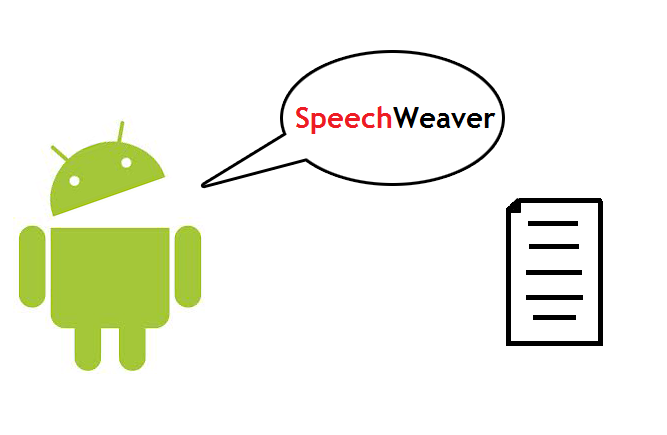
\includegraphics[width = 400pt, keepaspectratio = true]{fig/tempframsida3}

\begin{flushleft}
	{\noindent {\Huge Annotating Software Requirement Specifications with Mobile Speech Recognition} \\[0.5cm]
	\emph{\Large Master of Science Thesis in the Master Degree Programme Software Engineering} \\[.8cm]
	
	{\huge OLA PETERSSON}\\[.8cm]
    {\huge VIKTOR MELLGREN}\\[.8cm]
	
    
	{\Large Department of Software Engineering \\
	\textsc{Chalmers University of Technology} \\
	Gothenburg, Sweden 2013 \\
	Master's Thesis 2013:1\\
	}
    }
\end{flushleft}

\end{titlepage}
\ClearShipoutPicture
% End Chalmers title page

\pagestyle{empty}
%\newpage
%\clearpage
%\mbox{} 
%\newpage
\clearpage 
\thispagestyle{empty}

\begin{flushleft}
{\noindent
The Author grants to Chalmers University of Technology and University of Gothenburg
the non-exclusive right to publish the Work electronically and in a non-commercial
purpose make it accessible on the Internet. The Author warrants that he/she is the author
to the Work, and warrants that the Work does not contain text, pictures or other material
that violates copyright law.
 
The Author shall, when transferring the rights of the Work to a third party (for example
a publisher or a company), acknowledge the third party about this agreement. If the
Author has signed a copyright agreement with a third party regarding the Work, the
Author warrants hereby that he/she has obtained any necessary permission from this
third party to let Chalmers University of Technology and University of Gothenburg
store the Work electronically and make it accessible on the Internet.\\[.8cm]


\large{Annotating Software Requirement Specifications with Mobile Speech Recognition}\\[.2cm]
 
\null
\\

\uppercase{Ola Petersson},\\
\uppercase{Viktor Mellgren},\\[.2cm]
\null

\copyright \uppercase{Ola Petersson}, June 2013.\\
\copyright \uppercase{Viktor Mellgren}, June 2013. \\[.2cm]
 
Examiner: SVEN-ARNE ANDREASSON \\
Supervisor: \uppercase{ROBERT FELDT} \\[.2cm]
 
Chalmers University of Technology\\
University of Gothenburg\\
Department of Software Engineering\\
SE-412 96 Gothenburg\\
Sweden\\
Telephone + 46 (0)31-772 1000\\
\\
\null
\vfill
 Cover: The Android robot speaking to a document\\
    \null
    \\
Department of Software Engineering\\
Gothenburg, Sweden June 2013\\
}
\end{flushleft}

\pagestyle{empty}
\clearpage 
\thispagestyle{empty}

\begin{abstract}
Requirements are crucial in software engineering and there is ample support
for how to elicit and document them; however, relatively little support exist
for requirements maintenance. We argue that lightweight methods for annotating
requirements are needed and present a system based on speech recognition to
enable it. This paper describes the system design and a set of experiments and
user tests to validate its use. For more realistic evaluation our system has
been adapted to the commercial requirements management tool SystemWeaver.
Results show that the accuracy of free text speech input is not high enough to
enable free-form addition and edits to requirements. However, requirements
identification and annotation is practical by extending the system with 
string distance calculations to the set of requirements being matched. Lookup times on industrial
requirements data was deemed practical in
user tests, in particular for annotations on the go and during requirement reviews.
\\
\\
\smallskip
\noindent{\textbf{Keywords}: requirements engineering, speech recognition, lightweight, annotations, quality assurance, documentation, maintenance, mobile software, Android}
\end{abstract}

\pagestyle{empty}
\clearpage 
\thispagestyle{empty}

\section*{Acknowledgements}
We would like to thank Systemite AB for their cooperation, help and engagement in this thesis. Moreover, we would like to thank our supervisor Robert Feldt. Without you the thesis would not have been what it is today. We would also like to thank whoever coined the expression "how much wood could a woodchuck chuck if a woodchuck could chuck wood". It has been a tremendous help during our many hours of testing and evaluation of the speech recognizer. Finally, we thank our friends and family for their love and support. \\[1cm]
\hfill - Ola Petersson \& Viktor Mellgren, Göteborg 13/05/15

\newpage
\clearpage
\thispagestyle{empty}

\newpage
\clearpage
\mbox{}